\subsection{Normed space. Banach space}

Kreyszig 2.2 Normed Space. Banach Space 
1 Easy but fundamental
3 Very useful inequality
4 See metric spaces for something similar there
5 The most important norm there is
7 Feel free to use properties of the p-metric that you know
8 Similar to 7
9
11 Very useful to check something is not a norm, indeed:
12
13 Examples of nonnormed spaces 
15 Easy equivalent property to boundedness

\begin{exercise}{1}
Show that the norm $\norm{x}$ of $x$ is the distance from $x$ to 0.
\end{exercise}
\begin{proof}
fill
\end{proof}

\begin{exercise}{3}
Prove that for arbitrary $x,y\in X$, $\absoluteValue{\norm{y}-\norm{x}}\leq \norm{y-x}$.
\end{exercise}
\begin{proof}
fill
\end{proof}

\begin{exercise}{4}
Show that we may replace (N2; $\norm{x}=0\iff x=0$) by $\norm{x}=0\Rightarrow x=0$ without altering the concept of a norm. Show that nonnegativity of a norm also follows from (N3; $\norm{\alpha x}=\absoluteValue{\alpha}\norm{x}$) and (N4; $\norm{x+y}\leq \norm{x}+\norm{y}$).
\end{exercise}
\begin{proof}
fill
\end{proof}

\begin{exercise}{5}
Show $\norm{x}=\left(\sum_{j=1}^n\absoluteValue{x_j}^2\right)^{1/2}$, for $x\in\R^n$ or $x\in\C^n$) defines a norm.
\end{exercise}
\begin{proof}
fill
\end{proof}

\begin{exercise}{7}
Verify that $\norm{x}=\left(\sum_{j=1}^n\absoluteValue{x_j}^p\right)^{1/p}$ is a norm on the $l^p$ space.
\end{exercise}
\begin{proof}
fill
\end{proof}

\begin{exercise}{8}
There are several norms of practical importance on the vector space of ordered $n$-tuples of numbers (cf. 2.2-2), notably those defined by
\begin{align*}
    &\norm{x}_1 = \absoluteValue{x_1}+\absoluteValue{x_2}+\dots+\absoluteValue{x_n}\\
    &\norm{x}_p = (\absoluteValue{x_1}^p+\absoluteValue{x_2}^p+\dots+\absoluteValue{x_n}^p)^{1/p}\quad (1<p<\infty)\\
    &\norm{x}_\infty = \max[\absoluteValue{x_1},\dots,\absoluteValue{x_n}].
\end{align*}
In each case, verify that they are norms.
\end{exercise}
\begin{proof}
fill
\end{proof}

\begin{exercise}{9}
Verify that $\norm{x}=\max_{t\in [a,b]}\absoluteValue{x(t)}$ is a norm in $C[a,b]$.
\end{exercise}
\begin{proof}
fill
\end{proof}

\begin{exercise}{11 (Convex set, segment)}
fill
\end{exercise}
\begin{proof}
fill
\end{proof}

\begin{exercise}{12}
Using exercise 11, show that $\phi(x)=(\sqrt{\absoluteValue{x_1}}+\sqrt{\absoluteValue{x_2}})^2$ does not define a norm on the vector space of all ordered pairs $x=(x_1,x_2)$, of real numbers. Sketch the curve $\phi(x)=1$ and compare it with \Cref{fig:sec2-2-ex12}
\begin{figure}[H]
    \centering
    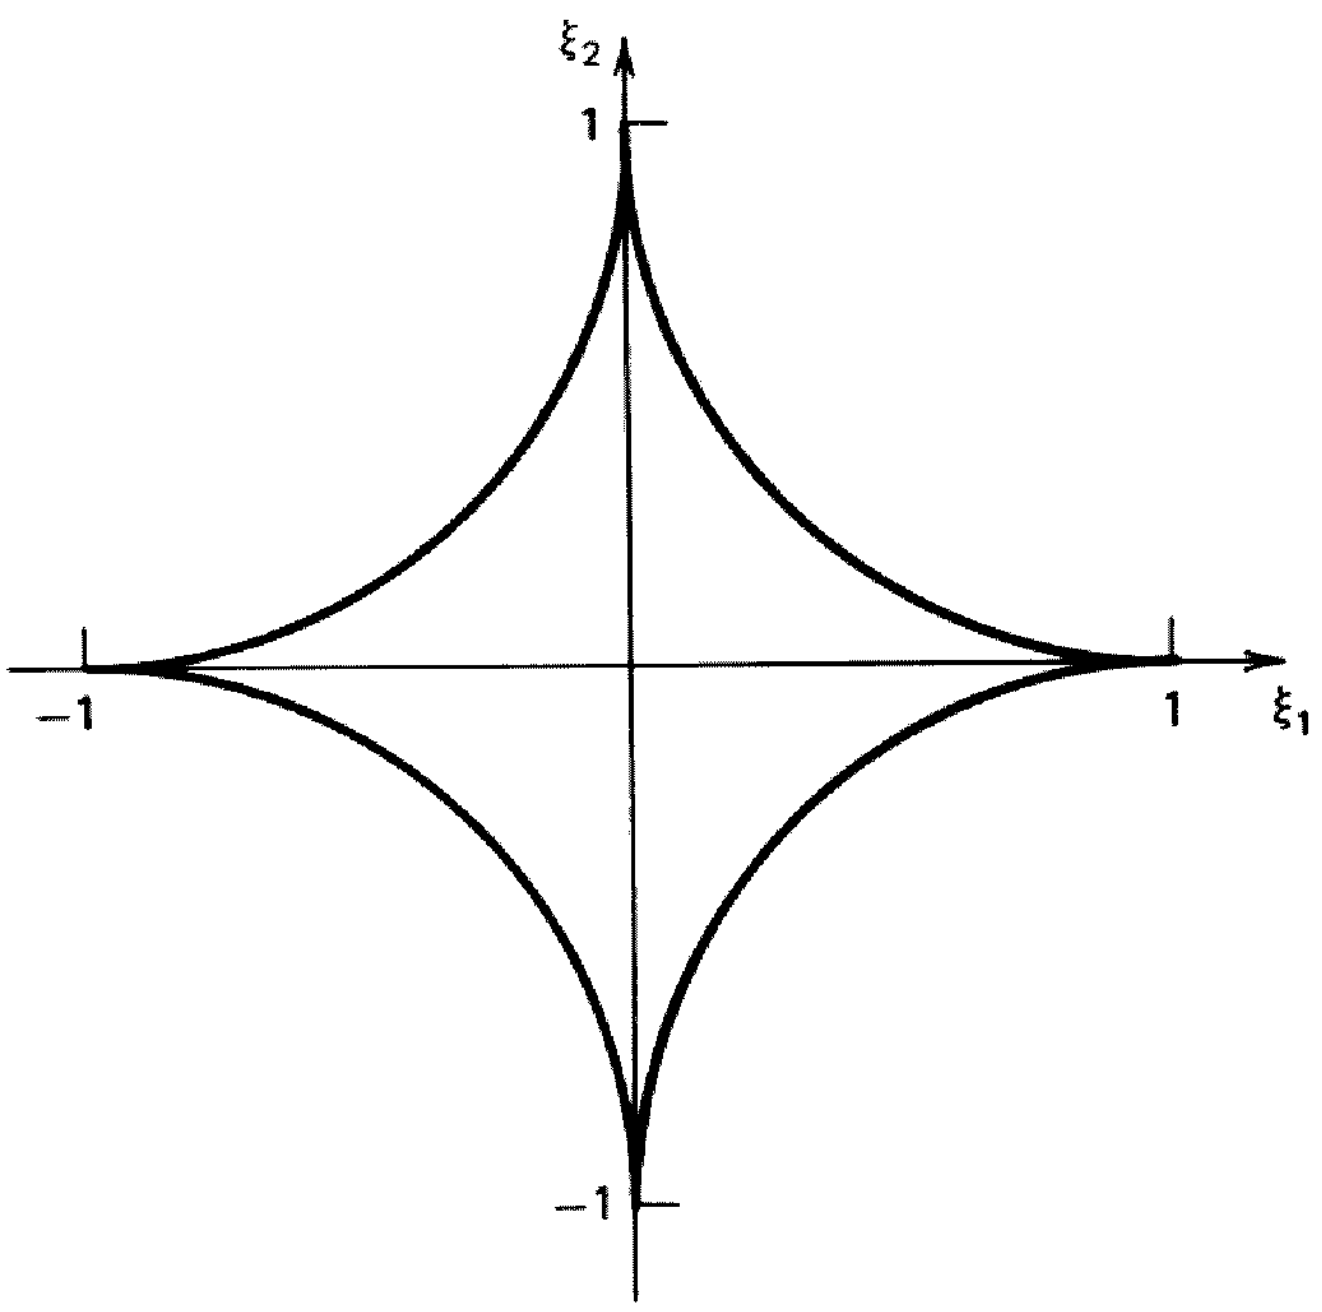
\includegraphics[width=0.5\textwidth]{kreyszig/assets/sec2-2-ex-12.png}
    \caption{Curve $\phi(x)=1$}
    \label{fig:sec2-2-ex12}
\end{figure}
\end{exercise}
\begin{proof}
fill
\end{proof}

\begin{exercise}{13}
fill
\end{exercise}
\begin{proof}
fill
\end{proof}

\begin{exercise}{15 (Bounded set)}
fill
\end{exercise}
\begin{proof}
fill
\end{proof}
